\documentclass[12pt]{article}
\usepackage{amssymb,amsthm,amsmath}
\usepackage[spanish]{babel}
\usepackage[latin1]{inputenc}
\usepackage{graphicx}

\begin{document}

En la revista \verb=trianguloscabri=, editada por el profesor
Ricardo Barroso de la Universidad de Sevilla, aparece el siguiente
problema (propuesto por Jos� Nogareda Villar, profesor de
matem�ticas del IES \lq\lq Ram�n Olleros de B�jar\rq\rq ,
Salamanca):

\begin{quote}
\textbf{137}. Sea $ABC$ un tri�ngulo. Sea $P$ un punto que no
pertenezca al mismo. Trazar por $P$ una recta de manera que corte
al tri�ngulo en dos figuras geom�tricas de la misma �rea.
\end{quote}

\begin{center}
\includegraphics{dibujo1.eps}
\end{center}

Asignamos coordenadas a los v�rtices del tri�ngulo $ABC$ de manera
que $A=(u,v)$, $B=(0,0)$ y $C=(c,0)$. Si $P=(x_0, y_0)$ es
cualquier punto del plano, una recta que pasa por $P$ tiene
ecuaci�n $y=y_0+ m(x-x_0)$. Llamaremos $E$ y $F$ a los puntos de
corte de esta recta con los lados $AB$ y $BC$, respectivamente.

\medskip Razonaremos que para muchos puntos $P$ puede encontrarse un
$m$ adecuado que permita calcular los puntos $E$ y $F$ cumpliendo
las condiciones del problema, y que para los dem�s $P$ podremos
encontrar puntos similares en los otros lados del tri�ngulo.

\medskip Un poco de c�lculo nos da las coordenadas de $E$ y $F$: \[
\begin{aligned}
  E =& \left( {\frac{{u(mx_0  - y_0 )}}
{{mu - v}},\frac{{v(mx_0  - y_0 )}} {{mu - v}}} \right), \hfill \\
  F =& \left( {x_0  - \frac{{y_0 }}
{m},0} \right).
\end{aligned}
\]

Usando que el �rea del tri�ngulo de v�rtices $(x_1,y_1)$,
$(x_2,y_2)$, $(x_3,x_3)$, viene dada por \[ \Delta  = \frac{1}
{2}\left| {\begin{array}{*{20}c}
   1 & 1 & 1  \\
   {x_1 } & {x_2 } & {x_3 }  \\
   {y_1 } & {y_2 } & {y_3 }  \\
 \end{array} } \right|,
\] obtenemos que \[
(EBF) = \frac{{v(y_0  - mx_0 )^2 }} {{2m(v - mu)}}.
\] y como debe ser $(EBF)= \frac{c v}{4}$, resolviendo, obtenemos dos
posibles valores de $m$: \[ m=\frac{{ - cv + 4x_0 y_0  \pm \sqrt c
\sqrt {cv^2  - 8vx_0 y_0  + 8uy_0^2 } }} {{2(2x_0^2  - cu)}}
\]

La figura siguiente muestra en color azul las posibles posiciones
del punto $P$ para que exactamente uno de estos valores de $m$
corresponda a una soluci�n del problema. En la regi�n amarilla
estar�an los puntos $P$ para los que las dos soluciones son
v�lidas.

\begin{center}
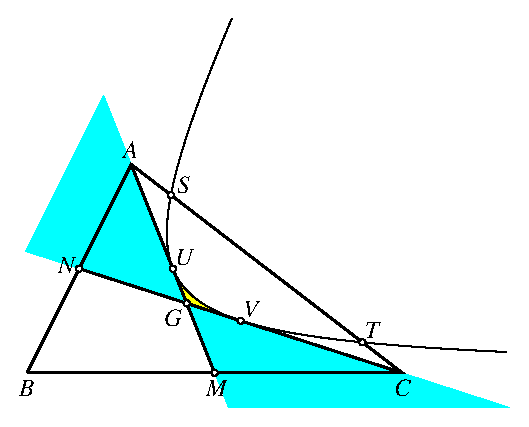
\includegraphics{dibujo2.eps}
\end{center}
La curva es una hip�rbola que tiene por as�ntotas a las rectas de
los lados $AB$ y $BC$, y que es tangente a las medianas del
tri�ngulo. La ecuaci�n de esta hip�rbola es la que aparece en el
radicando de la f�rmula de $m$, es decir $cv^2  - 8vx_0 y_0  +
8uy_0^2 = 0$.

\medskip Para dibujar esta hip�rbola de una forma sencilla con
\emph{Cabri G�om�tre II} necesitamos cinco puntos. Haciendo la
intersecci�n de la hip�rbola con las medianas podemos hallar los
puntos de tangencia $U$ y $V$, para los que se cumplen
$y=\frac{v}{2}$ e $y=\frac{v}{4}$, respectivamente.

\medskip Tambi�n podemos calcular los puntos de intersecci�n de la
hip�rbola con el lado $AC$. En este caso resulta \[ y = \left(
{\frac{1} {2} \pm \frac{{\sqrt 2 }} {4}} \right)v,
\] y como $\frac{1}{4} \sqrt 2 v$ es la cuarta parte de la
diagonal de un cuadrado de lado $v$, para obtener los puntos $S$ y
$T$, trazamos una circunferencia con centro el punto medio de $AC$
y radio la cuarta parte de la diagonal de un cuadrado de lado
$AC$. Como es sabido, los puntos que, como $U$ y $V$, est�n
sim�tricamente situados en el segmento $AC$ respecto de su punto
medio se llaman \emph{isot�micos}.

\medskip Teniendo en cuenta que la hip�rbola es sim�trica respecto
de la bisectriz interior del �ngulo $B$, podemos hallar un quinto
punto hallando cualquier de los sim�tricos de los puntos $U$ y
$V$.

\medskip Por �ltimo, digamos que los puntos del plano que no
est�n en ninguna de las zonas coloreadas del plano estar�n en las
zonas correspondientes al permutar adecuadamente los v�rtices $A$,
$B$ y $C$, por lo que para cualquier punto $P$ del plano es
posible resolver el problema planteado.

\bigskip \hfill \begin{small}
\begin{tabular}{l}
  \texttt{Francisco Javier Garc�a Capit�n, 2004.} \\
  \texttt{pacoga@ctv.es}
\end{tabular}
\end{small}

\newpage

\begin{center}
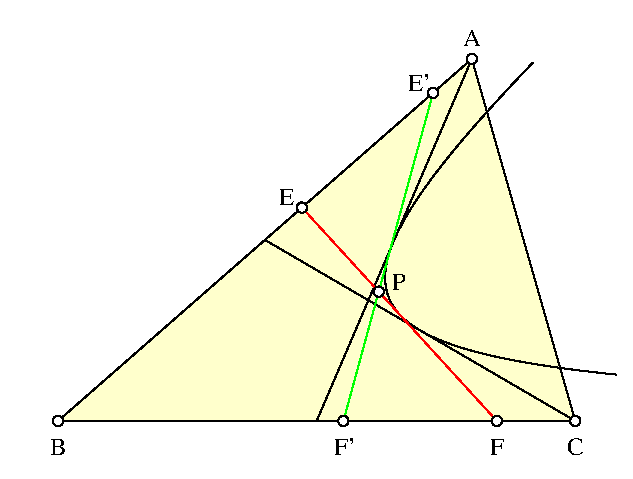
\includegraphics[scale=0.8]{137grafico1.eps}
\end{center}

\begin{center}
\includegraphics[scale=0.8]{137grafico2.eps}
\end{center}

\begin{center}
\includegraphics[scale=0.8]{137grafico3.eps}
\end{center}




\end{document}
